\chapter{Desarrollo}

En este capítulo se relata el proceso de desarrollo de esta aplicación web. Primero veremos la planificación inicial hablando de los diferentes artefactos que se generaron, posteriormente de cómo estos evolucionaron y se fueron adaptando, por último, del resultado final del desarrollo y lo aprendido en el camino.

\section{Arranque del desarrollo}

El primer artefacto que se generó es el Product Backlog, que recoge todas las funcionalidades deseadas por el equipo médico, en forma de historias de usuario (pequeños fragmentos de texto estructurado que intentan clarificar al máximo las mismas). Este se compone de una tabla con tres columnas: la primera de ellas recoge el grupo en el que se engloba la historia de usuario y su ID, la segunda una descripción corta de la misma y la última los criterios del comportamiento que debe tener la funcionalidad en los diversos escenarios posibles.
\newline

La generación de este artefacto fue compleja pues los médicos tenían claras dos o tres funcionalidades, que supondrán el núcleo de la aplicación (como veremos posteriormente). Del resto de la aplicación, o no tenían ninguna petición, o no había una opinión firme sobre ellas. Por ello, muchas de las funcionalidades de mediana o baja importancia fueron propuestas por el equipo de desarrollo o el director del TFG y el equipo médico se mostró más que contento de acogerlas prácticamente todas. A continuación se relatará y explicará cada sección de dicho Product Backlog y las modificaciones que sufrió. El documento completo en pdf para su cómoda lectura va adjunto a esta memoria.
\newpage

El núcleo del que hablábamos anteriormente, y por tanto lo primero a remarcar en nuestro Product Backlog, se compone de estas tres funcionalidades:
\newline

 \begin{figure}[h]
    \centering
     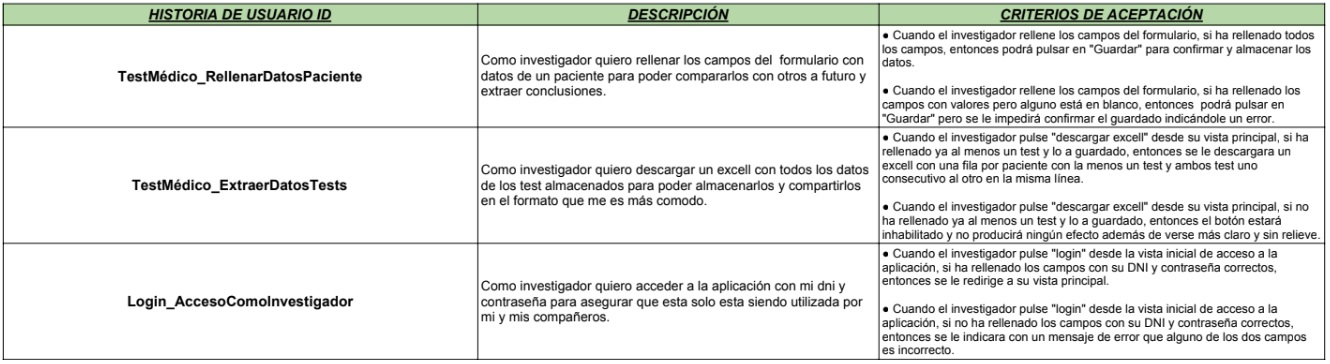
\includegraphics[width=1\textwidth]{images/historiasUsuario-1.jpg}
    \caption{Historias de usuario de mayor importancia, Walking Skeleton de la aplicación.}
\end{figure}


Como se puede apreciar en las historias de usuario lo principal era tener unos test donde rellenar los datos de los pacientes de forma cómoda, que estos datos pudieran luego ser extraídos en un Excel y que el acceso a la aplicación fuese privado a los miembros del equipo médico. Las dos primeras suponen la entrada y salida más básica de datos que permitiría al equipo médico extraer sus conclusiones y la tercera, a pesar de ser solo el login, el acceso a la aplicación, es también de gran importancia. Uno de los requisitos principales del estudio es el control de la procedencia y gestión de los datos. Únicamente pacientes que se hayan ofrecido voluntariamente vía formulario pueden tener sus datos representados y solo los miembros oficiales del estudio pueden tener acceso a ellos. Esto se consigue mediante un login cerrado que no permite ningún tipo de registro desde el exterior y la creación de todos los perfiles de investigador manualmente por el administrador.
\newpage

El siguiente bloque de funcionalidades complementa las tres primeras que en el primer prototipo emplearían perfiles introducidos a mano en la base de datos para probarse:
\newline

 \begin{figure}[h]
    \centering
     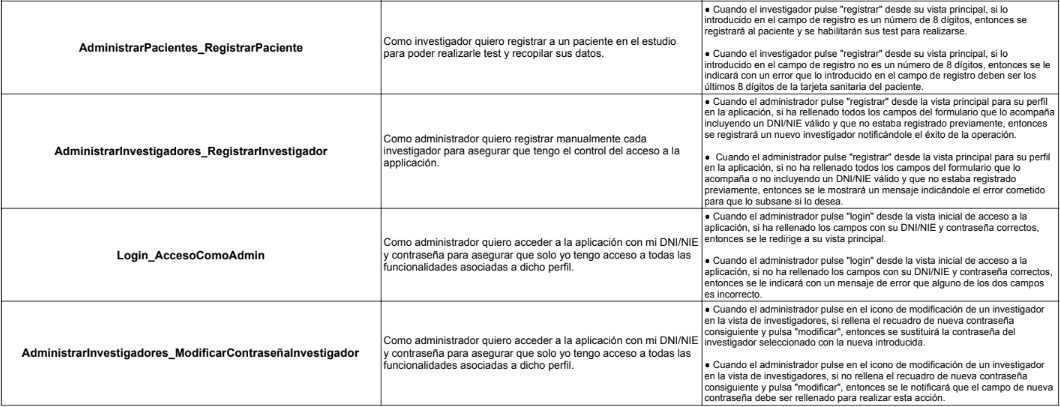
\includegraphics[width=1\textwidth]{images/historiasUsuario-2.jpg}
    \caption{Historias de usuario sobre la inclusión del perfil de administrador y los diversos registros.}
\end{figure}
\FloatBarrier


En este bloque se recogían los registros tanto de pacientes como investigadores así como el perfil de administrador y la modificación de contraseñas. Aparentemente, por lo explicado de parte del equipo médico, es un problema usual la pérdida de contraseña o el filtrado de las mismas por las condiciones de su ambiente de trabajo, y tener un acceso cómodo a su modificación es de gran importancia para ellos.
\newpage

Las funcionalidades que prosiguieron en la escala de valor para el cliente fueron las siguientes:
\newline

 \begin{figure}[h]
    \centering
     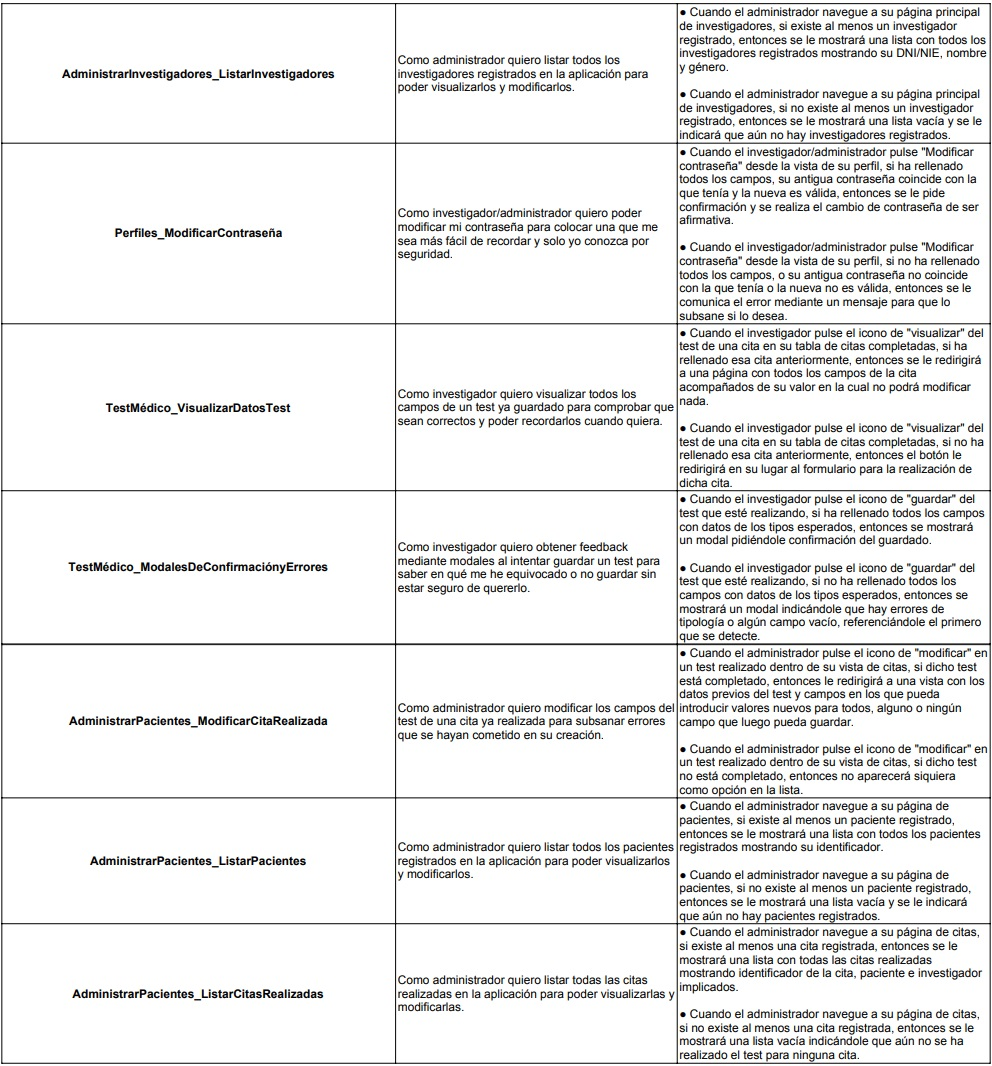
\includegraphics[width=1\textwidth]{images/historiasUsuario-3.jpg}
    \caption{Historias de usuario sobre listado de usuarios y diversas modificaciones.}
\end{figure}
\FloatBarrier


Estas funcionalidades se componen de dos tablas que listan de forma limpia tanto investigadores para el perfil de administrador, como pacientes para el de investigador. La funcionalidad de modificar contraseña de nuevo aparece, pero esta vez es para que cada investigador pueda cambiar su propia clave. Esta funcionalidad es principalmente para que el administrador pueda crear sus perfiles con contraseñas que ellos mismos puedan modificar al obtener las cuentas a algo fácil de recordar para ellos mismos. Además, se añade la posibilidad de visualizar en una plantilla los datos de un test realizado, ahorrando tener que extraer el Excel y consultarlo cada vez, cuando solo se quiere revisar el test de una cita en concreto. Se añaden modales para indicar errores y confirmación en los test, importante ya que estos no pueden ser modificados una vez guardados a no ser que lo haga el administrador manualmente. Esta posibilidad de modificar una cita por el administrador es la última funcionalidad no comentada de este bloque junto con su listar particular para facilitar el trabajo de este.
\newpage

El penúltimo bloque de funcionalidades que se extrajo al principio del desarrollo, empieza a corresponder ya a elementos de gestión necesarios pero no prioritarios que en su mayoría fueron propuestos por el equipo de desarrollo como posibles añadidos prácticos:
\newline

 \begin{figure}[h]
    \centering
     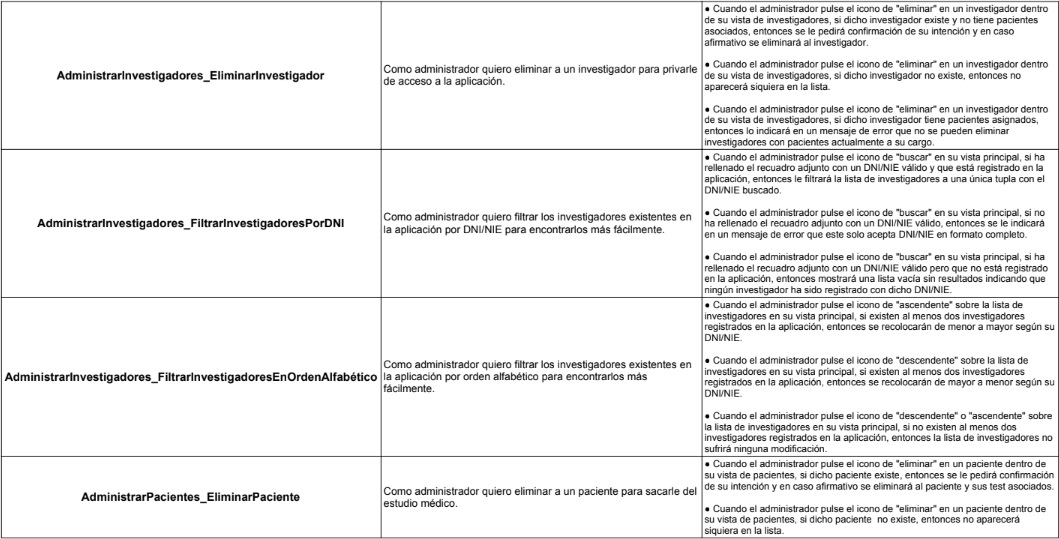
\includegraphics[width=1\textwidth]{images/historiasUsuario-4.jpg}
    \caption{Historias de usuario sobre eliminación de perfiles y agilidad en las búsquedas.}
\end{figure}

Como se puede observar, este bloque recogía principalmente la eliminación de perfiles, necesaria si algún paciente o investigador salía del proyecto. Esta funcionalidad, aunque simple, realmente no se añadió a este artefacto en un primer momento porque generaba dudas por la naturaleza del estudio. Los datos extraídos de la aplicación, para ser válidos, deben ser privados, de distintos periodos temporales y completos. La eliminación en este caso de un paciente podía dejar datos incompletos, o la de un investigador pacientes con citas a medio completar. Cualquiera de estos escenarios invalidaría el estudio. Por ello, en primera instancia, se pensó en no permitir ningún tipo de eliminación, pero tras debatir con el equipo médico este mismo aseguró que las eliminaciones serían pocas o prácticamente nulas y solo se usarían para subsanar erratas a la hora de crear perfiles nuevos sin afectar a los datos. Tras ello se decidió añadirlas, no sin delimitar claramente en sus criterios de aceptación las condiciones para poder realizar las eliminaciones.
\newline

La otra funcionalidad que apareció fueron los filtrados, los cuales habían sido implementados en otras aplicaciones por el equipo de desarrollo así que no suponían un gran esfuerzo y podían ser moderadamente útiles. Los médicos no se mostraron entusiastas con la idea pues apenas habría 15 investigadores pero ciertamente era una funcionalidad que podrían usar eventualmente así que se decidió añadirla.
\newpage

El último grupo de funcionalidades que cerraba este artefacto eran las menos prioritarias. Entre ellas un filtrado también para pacientes, la muestra de datos para cada investigador en su propio perfil y la inclusión de estadísticas. Esta última funcionalidad lamentablemente nunca pudo llevarse al desarrollo pues se prefirió cerrar la aplicación para poder tenerla funcionando y ajustarla a las necesidades del equipo médico a embarcarse en esta funcionalidad que nunca despertó mucho interés en el equipo:
\newline

 \begin{figure}[h]
    \centering
     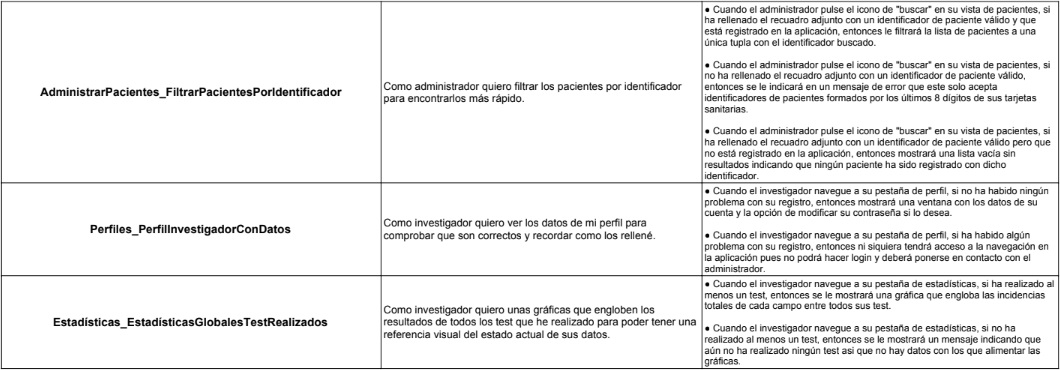
\includegraphics[width=1\textwidth]{images/historiasUsuario-5.jpg}
    \caption{Historias de usuario sobre filtrado de pacientes, perfiles de investigador y estadísticas.}
\end{figure}

Estas fueron todas las funcionalidades añadidas al Product Backlog al principio del desarrollo. En el siguiente apartado, el de desarrollo, se irán comentando los cambios que sufrieron estas historias y como aparecieron incluso algunas nuevas.
\newpage

Junto a este artefacto se creó también un User Story Map, que permite visualizar mejor todas las historias comentadas anteriormente y, además, marca un flujo de uso de las mismas de izquierda a derecha y secciona las funcionalidades en las releases mensuales en las que esperábamos tenerlas:
\newline

 \begin{figure}[h]
    \centering
     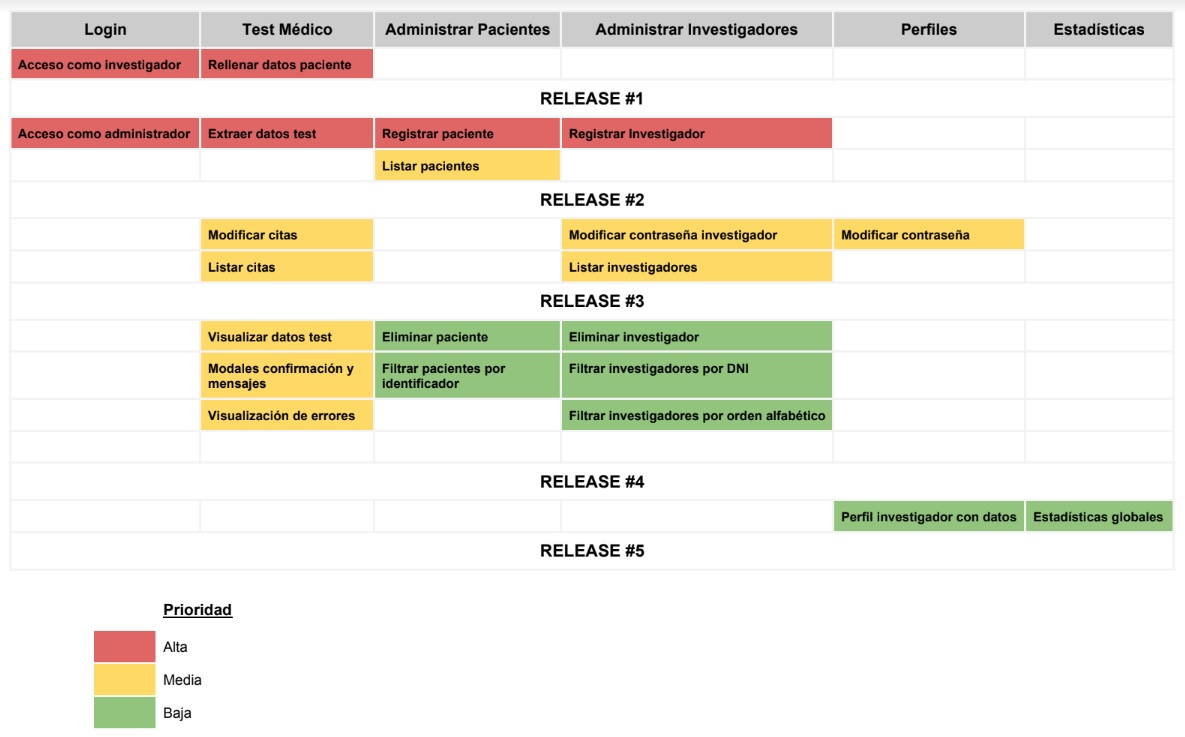
\includegraphics[width=1\textwidth]{images/userStoryMap.jpg}
    \caption{Mapa de historias de usuario.}
\end{figure}

Este mapa recoge todas las historias relatadas en este apartado y marca las divisiones en releases que seguirá el próximo para hablar de como fue el desarrollo de la aplicación, así que puede ser consultado en cualquier momento para clarificar de qué secciones de este apartado habla cualquier punto del desarrollo durante los sprints. Nótese que en ocasiones se hablará de sprints y en otras de releases, ya que en nuestro caso cada uno de los primeros coincide con una de las segundas.

\newpage

\section{Desarrollo durante los sprints}

Con nuestros artefactos listos y la primera reunión fijada para principios de octubre comenzó nuestro primer sprint en septiembre. Nuestro objetivo, como se puede apreciar en el User Story Map anterior, era el acceso a la aplicación como investigador y la posibilidad de rellenar tests de pacientes. La idea era empezar con el modelo de datos de los test, pensar en su extracción y después hacer el login, sin embargo, faltaban detalles sobre la estructura y limitaciones de los tests así que intercambiamos el orden a la espera de información más precisa. Visto lo cual comenzamos con el acceso a la aplicación.
\newline

A pesar de haber estado durante el mes de agosto viendo tutoriales y practicando con las tecnologías al ponernos de verdad sobre el proyecto comprobamos que aún teníamos que estudiar en profundidad muchos aspectos. Eduardo por suerte en el trabajo que había comenzado ese mismo verano había utilizado parte de las herramientas aunque no fuese en profundidad, pero Sergio no conocía herramientas como Angular o Spring Boot hasta hace un par de semanas. El primer mes se nos escapó de las manos prácticamente en configuración del software necesario y de los proyectos tanto en frontend como backend, la conexión de todo el sistema y el diseño de la simple página de login así como su funcionalidad. Para cuando llegó octubre el consumo de tareas iba mucho más lento de lo esperado y la primera reunión prácticamente solo sirvió para cerrar el diseño de la aplicación en líneas generales, la paleta de colores, el tipo de letra, el espaciado y tamaño, etc, y clarificar más detalles sobre el formulario de test para las citas. Este retraso en las tareas y desajuste del orden de desarrollo se mantendría lamentablemente para el siguiente sprint aunque se iría ajustando en los siguientes. A continuación se recoge una captura del login (ver figura 3.7).
\newline

 \begin{figure}[h]
    \centering
     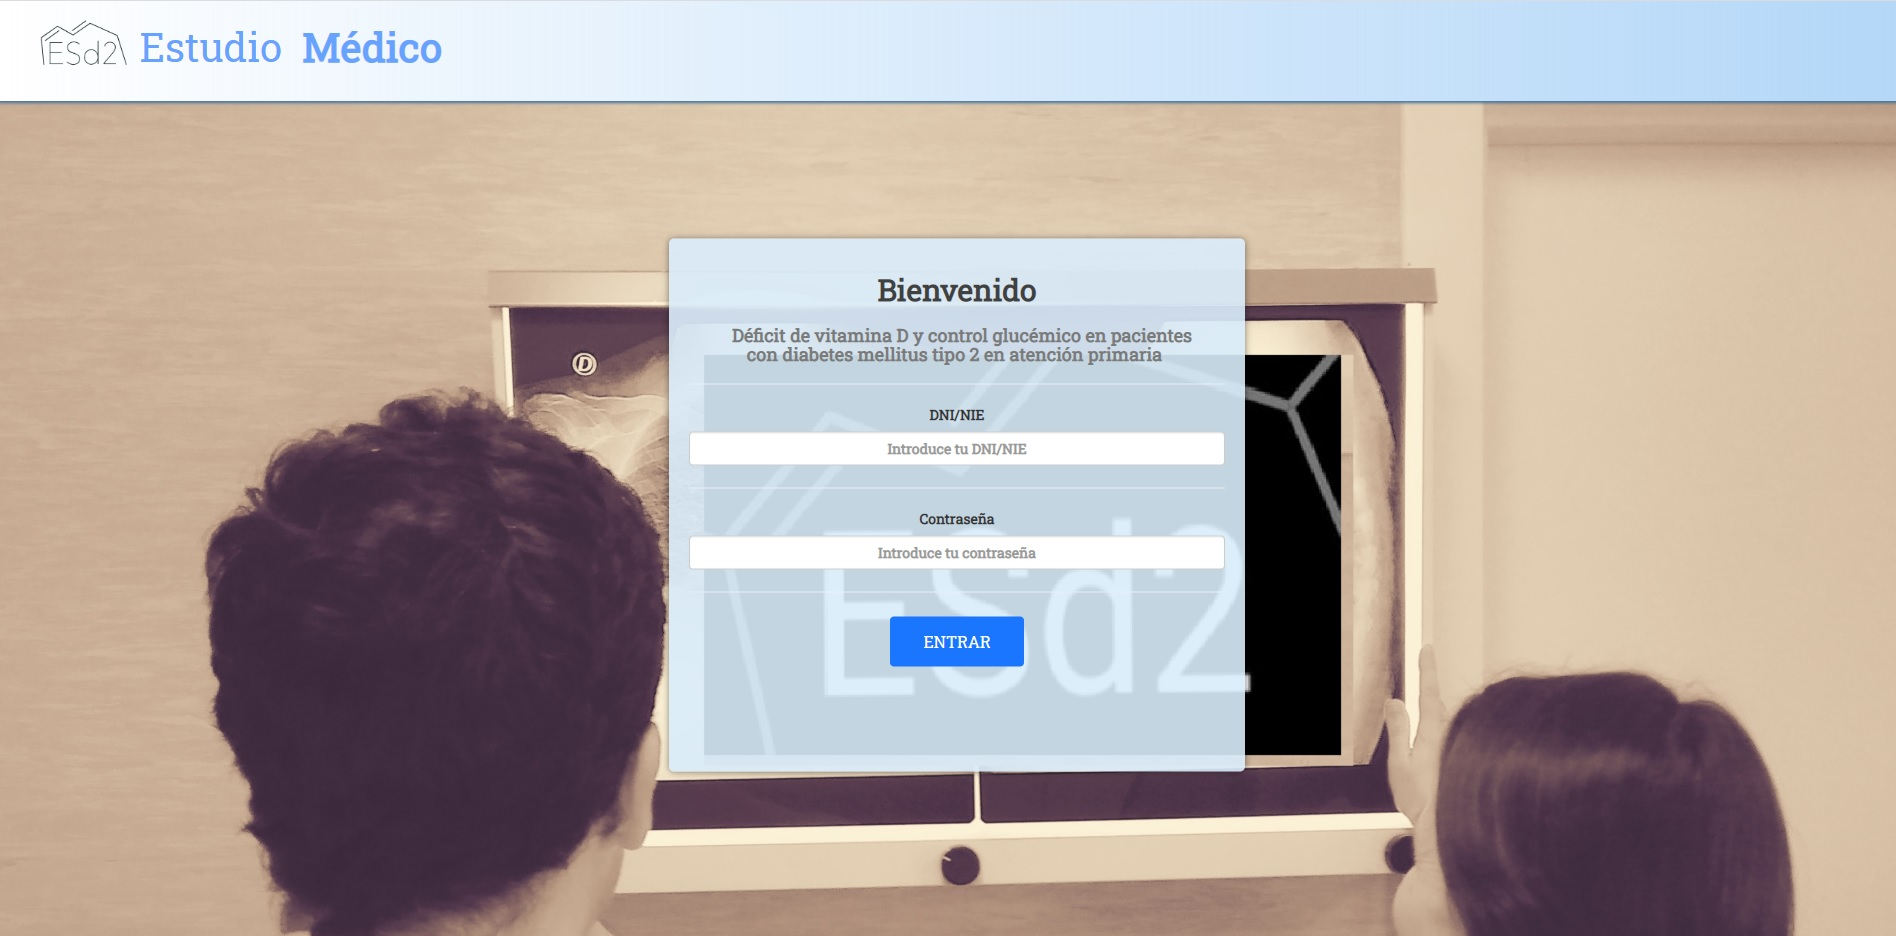
\includegraphics[width=1\textwidth]{images/login.jpg}
    \caption{Captura del login de la aplicación.}
\end{figure}
\newpage

Tras este primer sprint con retraso, el equipo de desarrollo al fin tenía todo listo y ordenado para trabajar en condiciones óptimas. Mientras Sergio se centraba en el formulario y el registro de pacientes, Eduardo pasó a las primeras tareas que no requerían el modelo de datos del test, el registro de investigadores y, a su vez, la creación y acceso del perfil de administrador. Al final de este segundo sprint el formulario estaba finalizado y los pacientes tenían su propio registro como se muestra en las siguientes figuras.
\newline

 \begin{figure}[h]
    \centering
     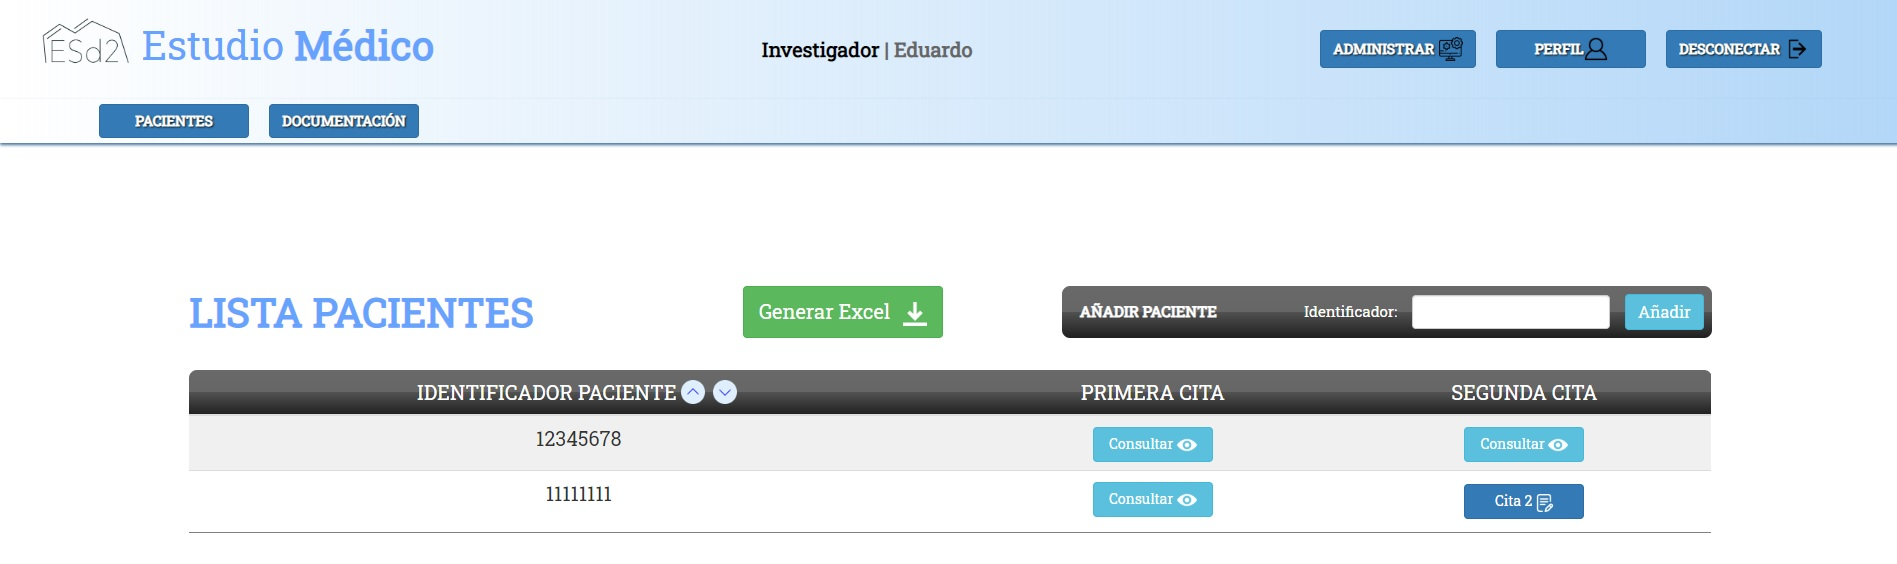
\includegraphics[width=1\textwidth]{images/investigadorPacientes.jpg}
    \caption{Vista principal del investigador con su lista de pacientes.}
\end{figure}

Esta captura (figura 3.8) muestra la imagen final de la vista principal del investigador con su lista de pacientes. En ese momento no existía aún el botón de generar Excel ni el de arriba a la derecha en el que se lee ``administrar''. Por lo demás el diseño se ideó y se mantuvo así desde un primer momento en toda la página a excepción de los iconos, que vendrían a futuro como un nuevo requisito.

\begin{figure}[h]
    \centering
     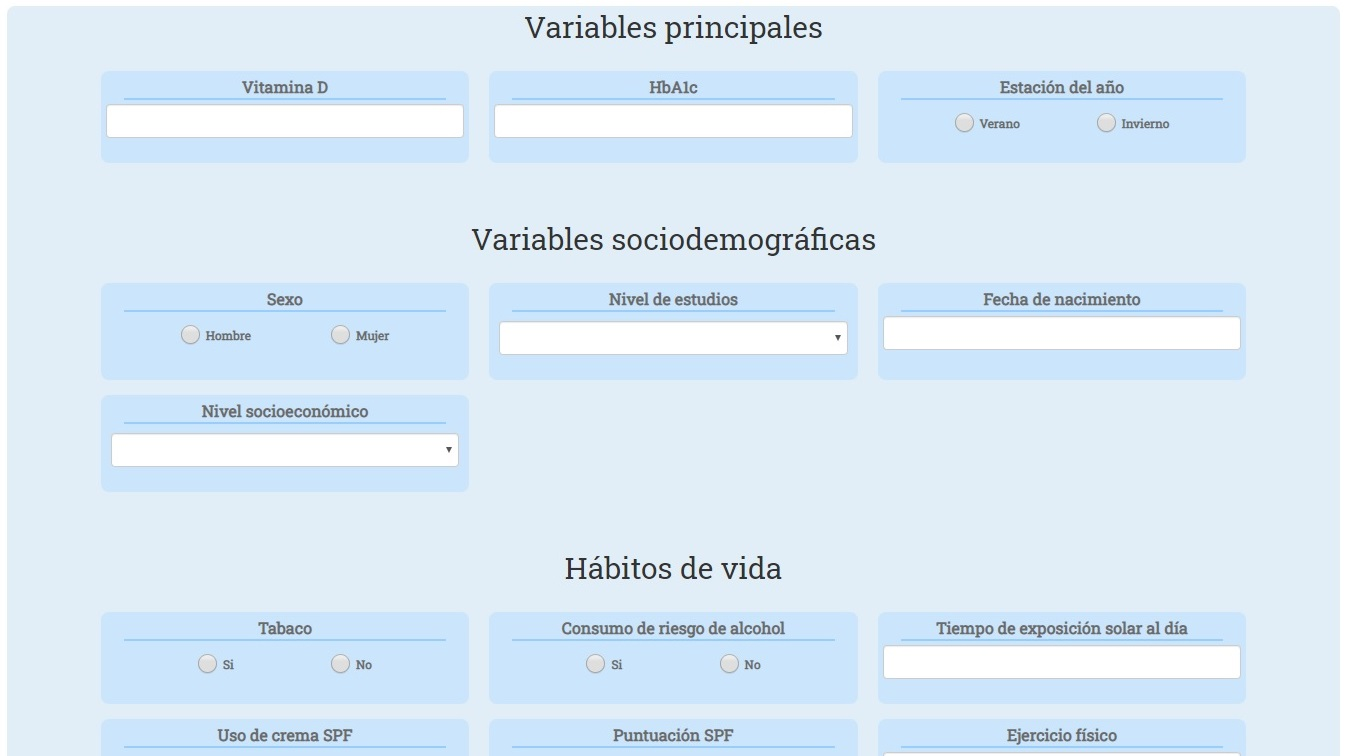
\includegraphics[width=1\textwidth]{images/testPacientes.jpg}
    \caption{Formulario de test para pacientes.}
\end{figure}

En cuanto al formulario, tanto el diseño como los campos (que eran imposible incluir en su totalidad en la figura 3.9) se crearon y mantuvieron como se ven en la figura anterior. Posteriormente se le añadirían algunas funcionalidades extra pero sin cambiar su aspecto.
\newpage

\begin{figure}[h]
    \centering
     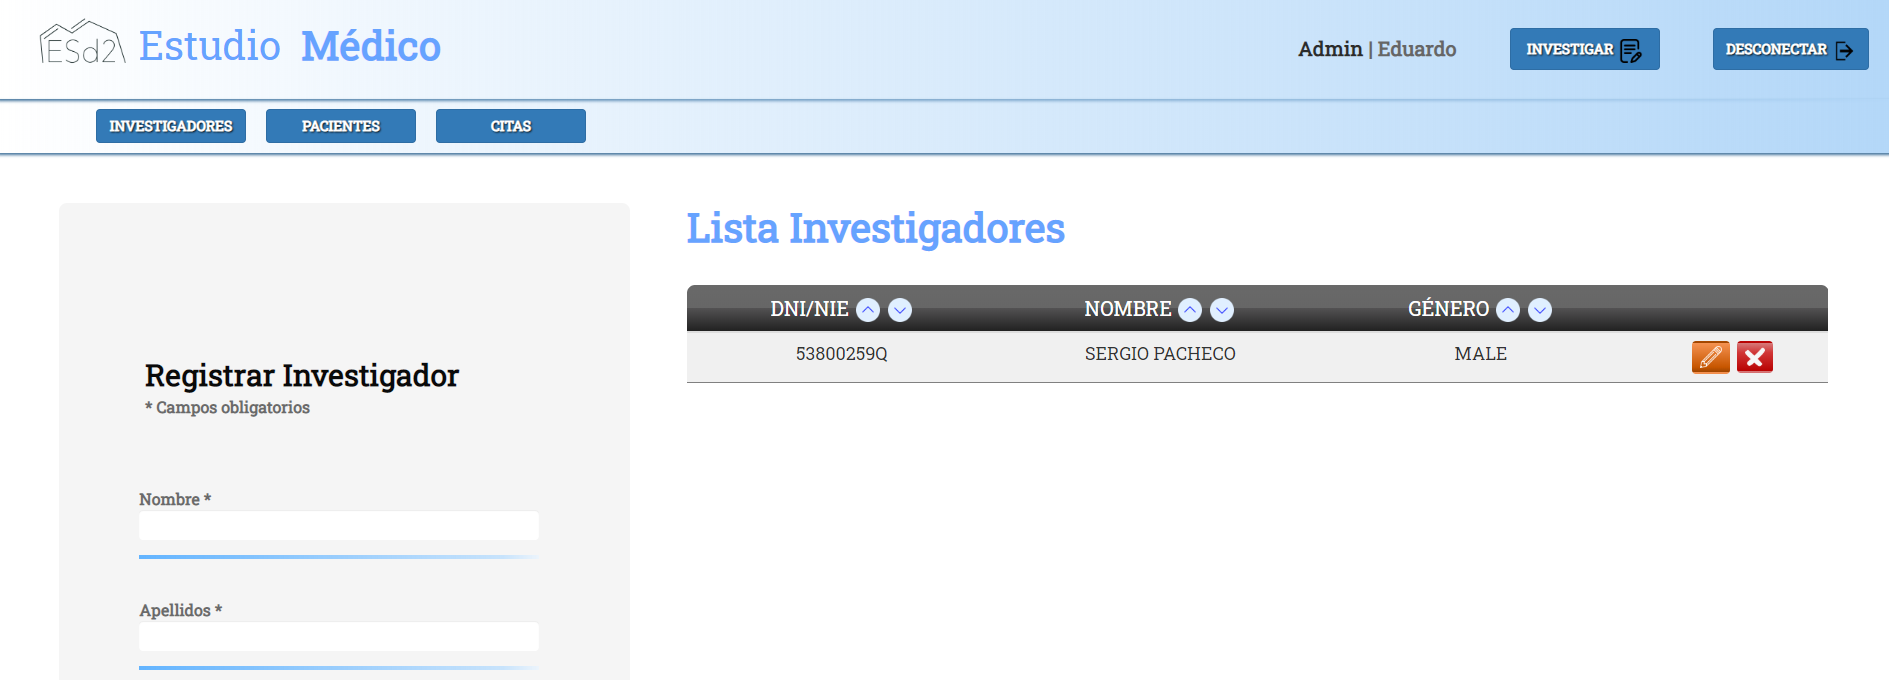
\includegraphics[width=1\textwidth]{images/adminInvestigadores.png}
    \caption{Vista principal del administrador con la lista de investigadores.}
\end{figure}

En la figura 3.10 se observa la lista de investigadores en la ventana principal de administrador, con el mismo diseño que la de pacientes pero con dos botones añadidos que permitirían posteriormente modificar la contraseña de investigador y eliminarlo. Al lado izquierdo se ve el formulario de registro de investigador que aparece completo en la figura 3.11.

\begin{figure}[h]
    \centering
     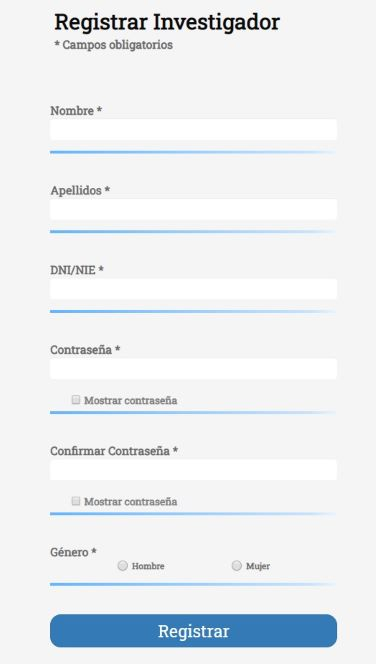
\includegraphics[width=6.cm,height=10.cm]{images/registrarInvestigadores.jpg}
    \caption{Formulario para registrar nuevos investigadores como administrador.}
\end{figure}
\newpage

Las claves de acceso a la aplicación son el DNI y la contraseña. Como se observa en la figura, se puede utilizar un NIE como clave, este detalle fue introducido a posteriori con el despliegue de la web ya que una de las investigadoras es extranjera.
\newline

Con estas funcionalidades implementadas, la segunda release se llevó a cabo con todas las tareas consumidas a excepción de la extracción de datos, que sería lo primero a retomar en el siguiente sprint. El equipo médico mostró conformidad con todo el desarrollo hasta la fecha aunque solicitó algunos añadidos para el formulario. Durante la demo realizada en la reunión el médico representante del equipo y codirector del TFG, Alejandro, notó que el formulario no daba indicaciones de qué valores se esperaban en los diferentes campos y no daba suficiente información de los errores. Los miembros del equipo de desarrollo no sabíamos nada acerca de qué valores serían válidos o la información que les seria útil en un mensaje de error en el formulario así que Alejandro recopiló por cuenta propia todos estos datos y nos los envió en un documento por correo al par de días.

\begin{figure}[h]
    \centering
     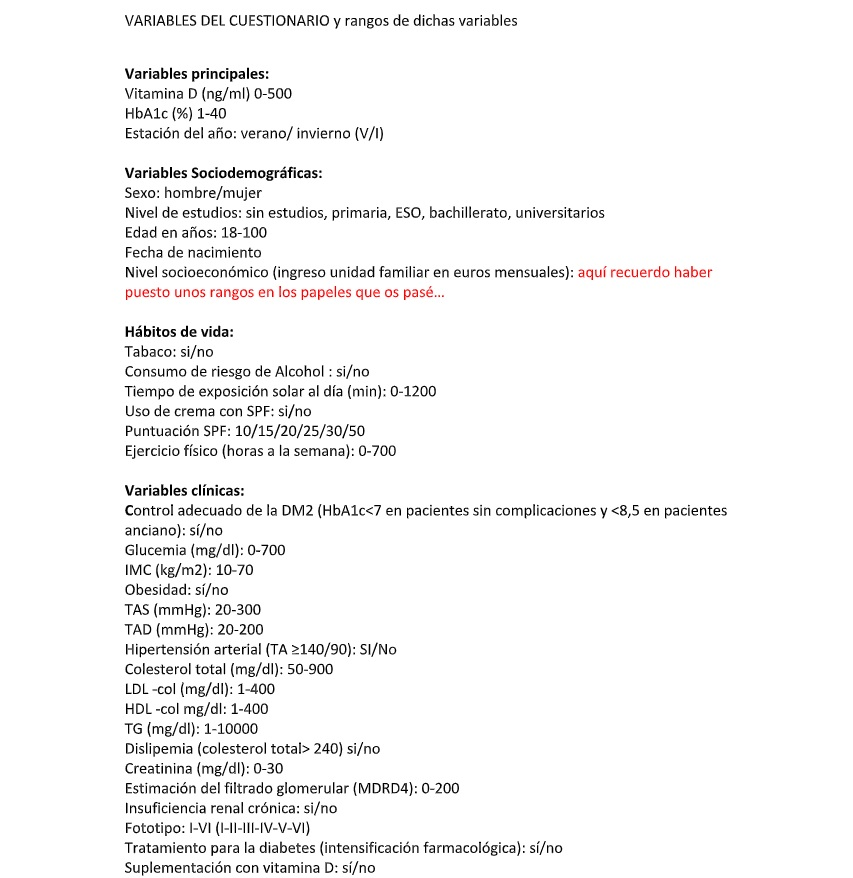
\includegraphics[width=1\textwidth]{images/rangosVariables.jpg}
    \caption{Documento con rangos de variables y tipo de campos esperados en el formulario.}
\end{figure}
\newpage

Estos valores se añadieron posteriormente al formulario en forma de tooltips, pequeños bocadillos de información al pasar el cursor sobre los nombres de cada campo del formulario.

\begin{figure}[h]
    \centering
     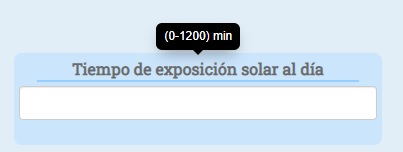
\includegraphics[width=1\textwidth]{images/tooltip.jpg}
    \caption{Tooltip de información sobre el rango de valores esperado en un campo del formulario.}
\end{figure}

Además se añadió un remarcado en rojo para cuando el valor estuviese fuera de ese rango o no fuese siquiera un número y uno en verde cuando el contenido del campo cumpliese los requisitos establecidos.

\begin{figure}[h]
    \centering
     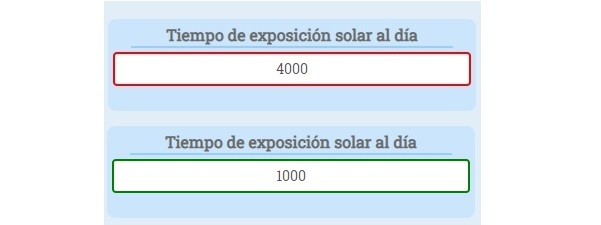
\includegraphics[width=1\textwidth]{images/remarcadoRojo.jpg}
    \caption{Remarcado de colores para visualizar si el valor cumple los requisitos del campo del formulario.}
\end{figure}
\newpage

En el siguiente sprint todas las funcionalidades se centraban en la modificación de los diferentes elementos de la aplicación, sin embargo tras hablar con el equipo médico se llevaron a cabo varios cambios en el orden de prioridad:

\begin{itemize}
    \item Las funcionalidades referentes al perfil (en este punto sobre todo la modificación de contraseña) se relegaron a una prioridad baja. Ciertamente la posibilidad de cambiar la contraseña por el usuario era importante para los médicos pero no más que la visualización de los datos del formulario o las funcionalidades aún restantes de gestión para los usuarios.\newline
    
    \item Relacionado con lo dicho en el punto anterior, eliminar perfiles y filtros pasaron a una prioridad media y se pusieron al nivel de visualizar datos test. Estas historias de usuario pasaron a la release 3.\newline
    
    \item En cuanto a la historia de modificar citas y listarlas, estas mantuvieron su prioridad, pero su carga de trabajo, con todos los nuevos detalles de rangos y validaciones añadidos al formulario, se había vuelto abrumadora. El equipo lo comentó con el representante de los médicos y este dio el visto bueno a posponerla ya que era una herramienta de corrección de errores y todo nuestro trabajo en el momento sobre el formulario se encaminaba a la prevención de los mismos al máximo.\newline
    
    \begin{figure}[h]
    \centering
     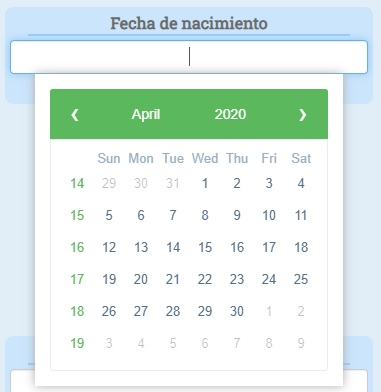
\includegraphics[width=7.cm,height=7.cm]{images/calendario.jpg}
    \caption{Calendario mejorado, mucho más fácil de manejar que escribir la fecha manualmente, lo que llevaba a errores.}
    \end{figure}
    
    \item Por último, aunque no se añadiese una nueva, se mantuvo abierta la historia de rellenar datos paciente ya que durante todo este sprint se siguió trabajando en mejoras para el mismo y detalles que se iban comentando por correo con el equipo médico. \newline
\end{itemize}
\newpage

Con esta nueva organización se continuó con el desarrollo. La historia de ``Modificar contraseña investigador'' se amplió, ya que suponía poco trabajo extra y resultaba interesante, a modificación de cualquier campo del investigador.

\begin{figure}[h]
    \centering
     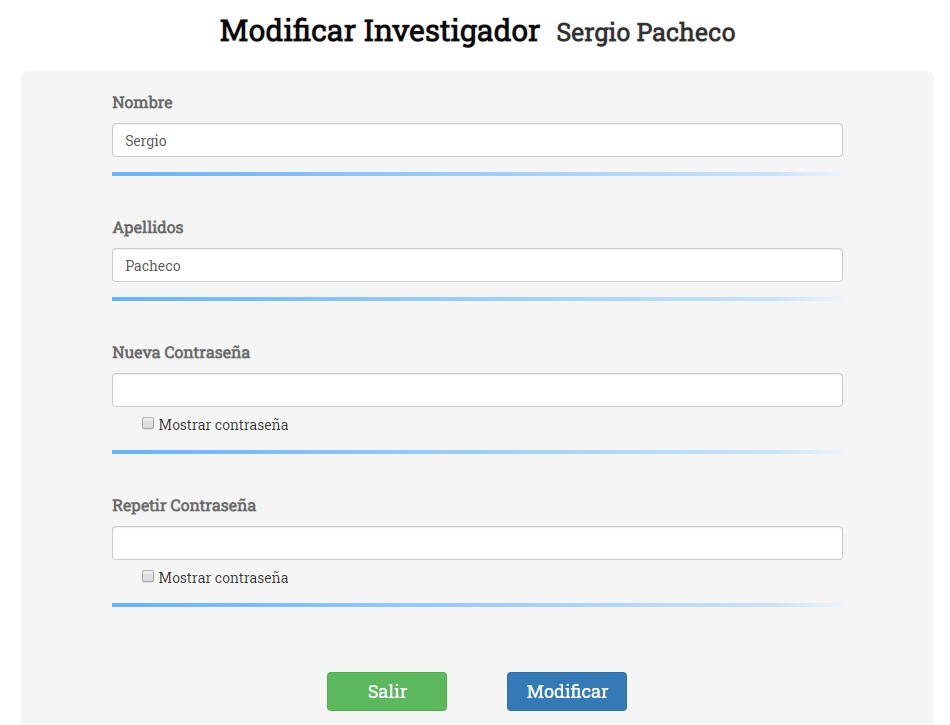
\includegraphics[width=1\textwidth]{images/modificarInvestigador.jpg}
    \caption{Formulario para la modificación de datos de un investigador por parte del administrador.}
\end{figure}

Los listar, tanto pacientes como investigadores, fueron finalizados y junto con otros elementos visuales rediseñados para incluir iconos. Estos iconos fueron una propuesta del profesor director en la que nunca se pensó pero que ciertamente añadían usabilidad a la interfaz general de la aplicación.\newline

En cuanto a la eliminación de perfiles, como se comentó en el punto de arranque del proyecto no está permitido eliminar investigadores con pacientes asignados y los pacientes pueden eliminarse tengan o no citas realizadas, pero en el caso de tenerlas se pedirá una confirmación extra para evitar posibles problemas. En caso de confirmar la eliminación, sus citas completadas por el momento, así como el perfil del pacientes serán eliminadas de la base de datos.

\begin{figure}[h]
    \centering
     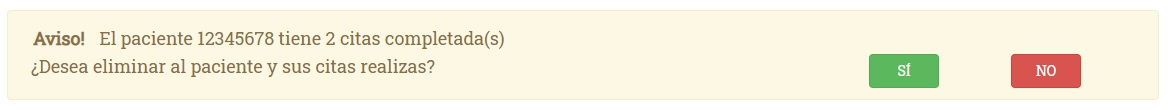
\includegraphics[width=1\textwidth]{images/confirmacionEliminarPaciente.jpg}
    \caption{Mensaje de confirmación para la eliminación de un paciente con algún test de sus citas relleno.}
\end{figure}
\newpage

Se añadieron los filtros tanto para pacientes como para investigadores. En el caso de los investigadores se sometió a debate la posibilidad de implementar una lista desplegable en vez de un buscador por DNI escrito, pero el numero de investigadores (unos 15) dejaba la lista algo larga como para ser cómoda y el buscador algo amplio para ser tan pocos. Finalmente, se decantó por el buscador, principalmente por mantener una concordancia y similitud con el sistema empleado para los pacientes.

\begin{figure}[h]
    \centering
     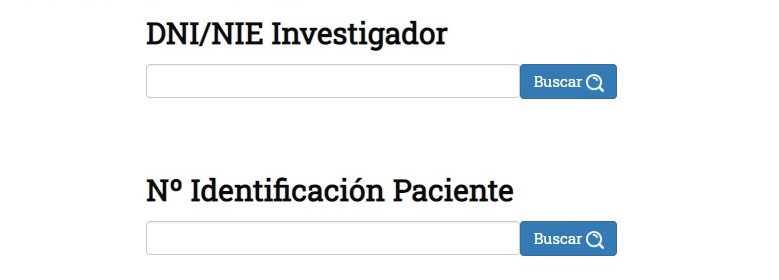
\includegraphics[width=1\textwidth]{images/filtros.jpg}
    \caption{Filtros para la búsqueda por DNI de investigador o identificador de paciente.}
\end{figure}

Terminada esta tercera release, la reunión con el representante del equipo médico y el profesor director del TFG se llevó a cabo. En cuanto al formulario de test para las citas, quedó cerrado a excepción de un pequeño añadido que hizo ver el profesor: en los campos que puedan admitir o no decimales el mensaje de información sobre su contenido debería clarificarlo. Por la parte de gestiones de usuarios tanto modificación, eliminación o filtrado no hubo ninguna queja, aunque era de esperar pues sus condiciones ya habían sido habladas múltiples veces tanto de forma presencial como por email. Con todo revisado y los detalles de algunas historias apuntados se procedió con el cuarto sprint, el último, con una gran carga de tareas.
\newline

Finalmente, se llevó a cabo la extracción de datos de la aplicación a un Excel. En un primer momento se hizo dejando una línea para cada cita de cada paciente, pero por petición del equipo médico tras ver el resultado se modificó a una sola línea por paciente con sus dos citas consecutivas en la misma.

\begin{figure}[h]
    \centering
     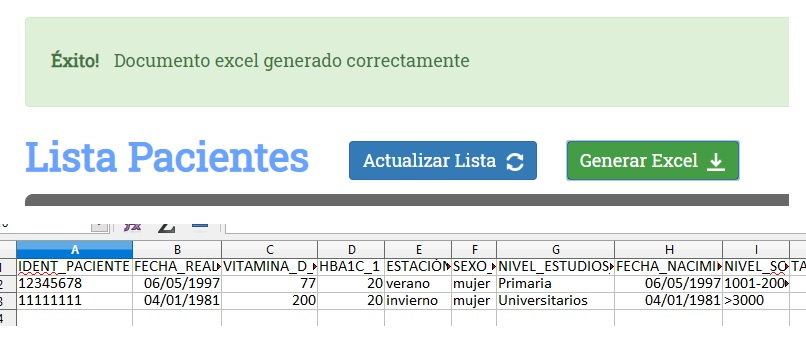
\includegraphics[width=1\textwidth]{images/extraerDatos.jpg}
    \caption{Mensaje de confirmación de la extracción de datos y documento Excel resultante.}
\end{figure}
\newpage

La visualización de los datos del test se implementó siguiendo el diseño del formulario de recopilación de datos pero listando los campos para facilitar su lectura. Además, se mantuvieron los tooltip para permitir su consulta en todo momento y no ofuscar ninguna información.

\begin{figure}[h]
    \centering
     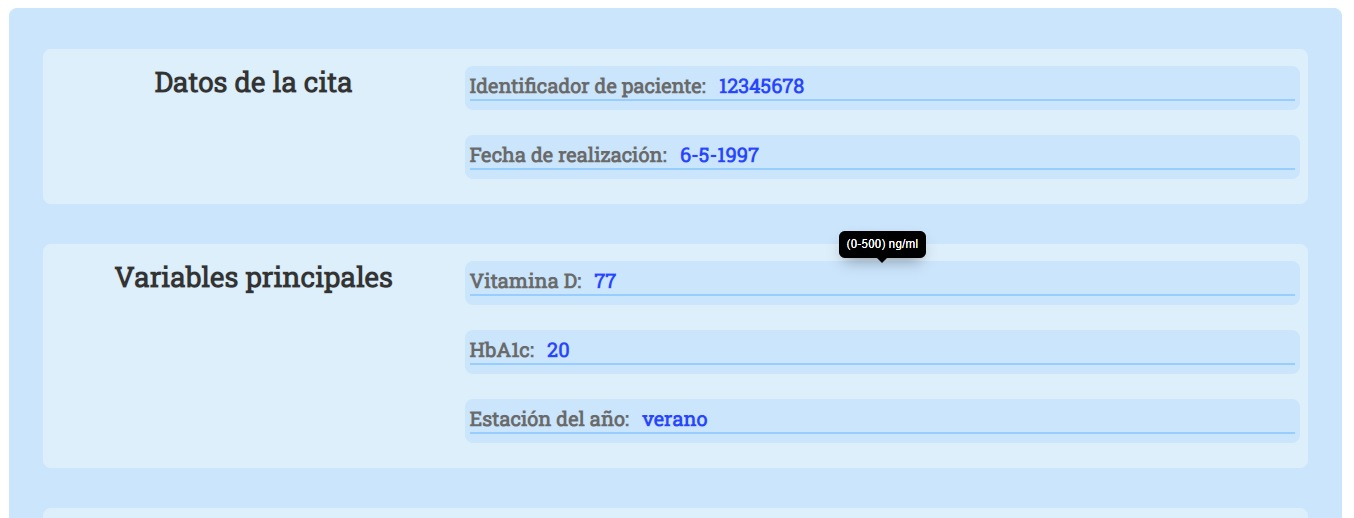
\includegraphics[width=1\textwidth]{images/visualizarTest.jpg}
    \caption{Fragmento de la visualización de un test realizado.}
\end{figure}

Se añadieron y mejoraron mensajes de error y modales de confirmación para la inserción de datos en la aplicación, ya fuese de usuario o de los propios test sobre pacientes.

\begin{figure}[h]
    \centering
     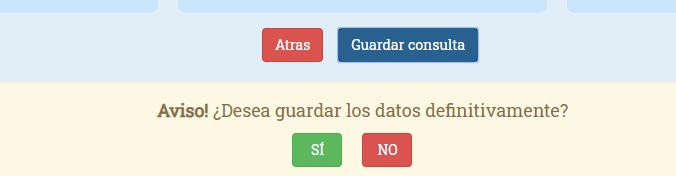
\includegraphics[width=1\textwidth]{images/modales.jpg}
    \caption{Modal de confirmación para el guardado de un test.}
\end{figure}

Se cerraron todas las historias que aún acumulaban modificaciones hasta la fecha como \textit{Rellenar datos paciente} y se completaron ambas historias de la sección de \textit{Perfiles} con la modificación de contraseña propia para cada investigador y la visualización de sus datos.

\begin{figure}[h]
    \centering
     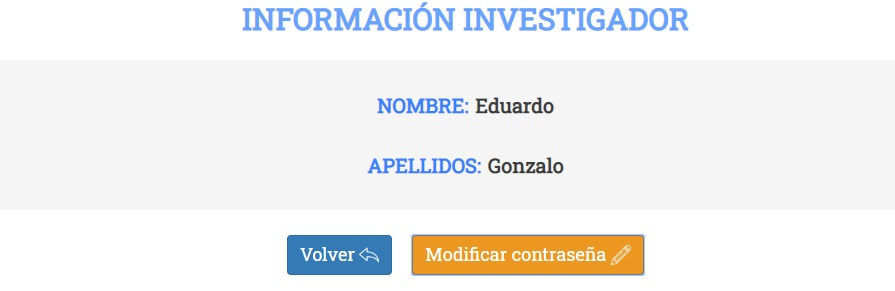
\includegraphics[width=14.cm,height=4.cm]{images/perfil.jpg}
    \caption{Perfil de investigador.}
\end{figure}
\newpage

Por último, en este sprint se llevó a cabo la implementación de las historias \textit{Modificar citas} y \textit{Listar citas}, que se llevaron una gran parte de la carga de trabajo del mismo. Para la lista de citas se decidió añadir una nueva historia de usuario \textit{Filtrar citas por identificador de paciente} para dar alguna herramienta de filtrado en esta lista que será presumiblemente la más larga. Además, se mantuvieron los filtros de menor a mayor ya implementados en anteriores listas. Se añadió un pequeño botón de actualización sobre la lista ya que las citas son los componentes más cambiantes de la aplicación y pueden estarse añadiendo frecuentemente al mismo tiempo que se consulta esta tabla. Para evitar que el usuario tenga que recargar la página para ver estos cambios y recordarle que pueden estarse sucediendo se añade este botón.

\begin{figure}[h]
    \centering
     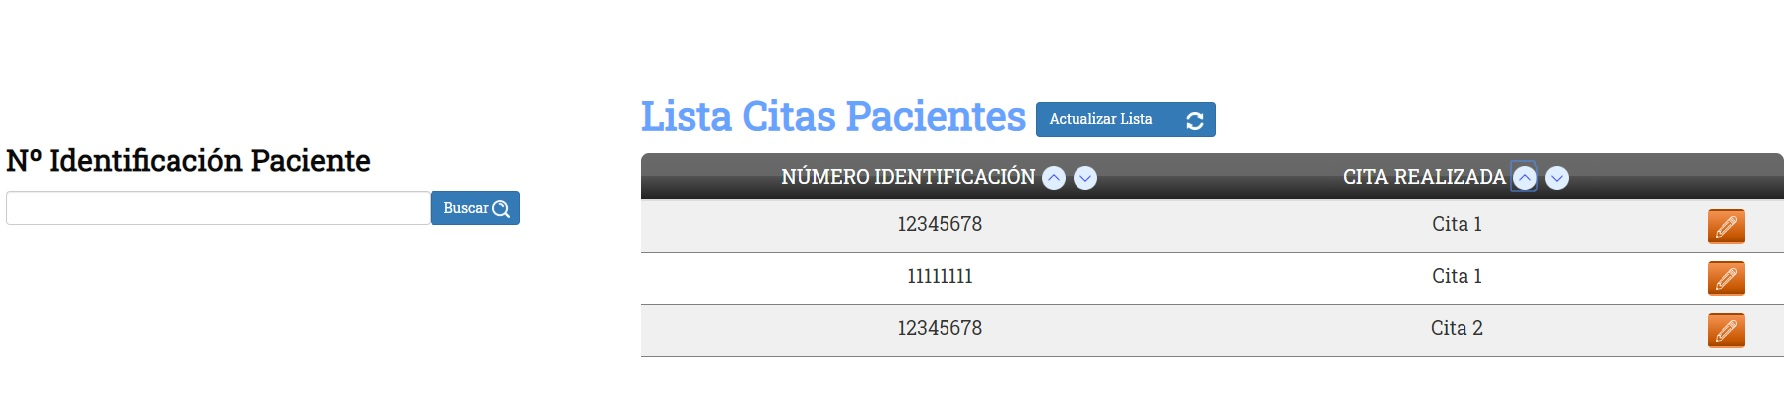
\includegraphics[width=1\textwidth]{images/listarCitas.jpg}
    \caption{Perfil de investigador.}
\end{figure}

En cuanto a la modificación de las citas por parte del administrador, se decidió mantener el estilo de la visualización de citas realizadas ya que era más compacto pero añadiendo campos para poder rellenar aquellos datos que quisieran modificarse. Estas modificaciones siguen los mismos criterios de entrada que el test original, reaccionan de igual manera con el patrón de colores a las inserciones válidas o inválidas y tienen los mismos mensajes de error, a excepción de que este formulario no requiere todos los campos rellenos.

\begin{figure}[h]
    \centering
     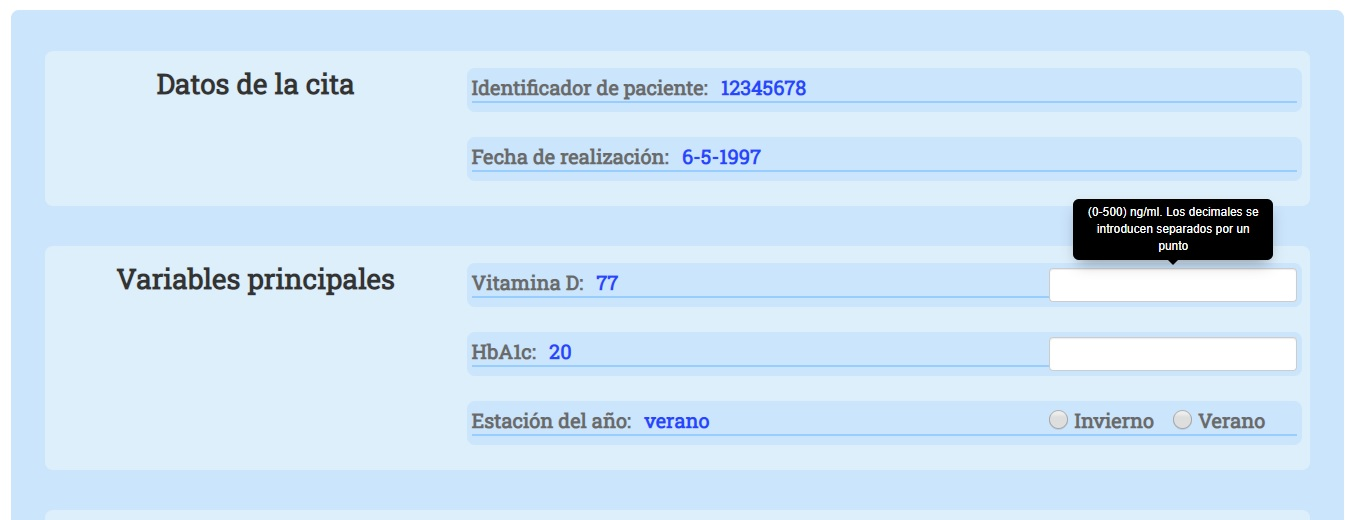
\includegraphics[width=1\textwidth]{images/modificarCita.jpg}
    \caption{Formulario de modificación para un test realizado sobre una cita.}
\end{figure}

Como se ha visto en las figuras y se recoge en el mapa de historias de usuario de la sección anterior, con esto quedaba completada la mayor parte de la aplicación. La ultima reunión en diciembre de 2019 se llevó a cabo y aunque la siguiente técnicamente debía ser a finales de enero con las festividades y los exámenes se tuvo que posponer a febrero. En vistas de las fechas que se manejaban ya, como se comentó anteriormente, se dejó de lado el apartado de estadísticas y se empezó a trabajar en el despliegue de la aplicación del que se hablará en un próximo capítulo. Además, los artefactos utilizados tanto para planificación como gestión se mantuvieron durante esta fase de despliegue, y tras esta, durante el mantenimiento del que igualmente se hablará en su propio capítulo.